\documentclass[12pt]{article}

% -------------------------------------------------
% Packages
% -------------------------------------------------

\usepackage[a4paper,margin=1in]{geometry}
\usepackage{booktabs}
\usepackage{listings}
\usepackage{xcolor}
\usepackage{amsmath}
\usepackage{graphicx}
\usepackage{float}
\usepackage{hyperref}
\usepackage{array}

% -------------------------------------------------
% Code Style
% -------------------------------------------------

\definecolor{codegreen}{rgb}{0,0.6,0}
\definecolor{codegray}{rgb}{0.5,0.5,0.5}
\definecolor{codepurple}{rgb}{0.58,0,0.82}
\definecolor{backcolour}{rgb}{0.95,0.95,0.92}

\lstdefinestyle{pythonstyle}{
    backgroundcolor=\color{backcolour},
    commentstyle=\color{codegreen},
    keywordstyle=\color{blue},
    stringstyle=\color{codepurple},
    numberstyle=\tiny\color{codegray},
    basicstyle=\ttfamily\small,
    numbers=left,
    numbersep=8pt,
    breaklines=true,
    showstringspaces=false,
    tabsize=4,
    language=Python
}

\lstset{style=pythonstyle}

% -------------------------------------------------
% Hyperlink Setup
% -------------------------------------------------

\hypersetup{
    colorlinks=true,
    linkcolor=blue,
    urlcolor=blue
}

% -------------------------------------------------
% Report Details
% -------------------------------------------------

\title{
    \textbf{Deep Learning Laboratory}\\
    \vspace{0.3cm}
    Assignment \#2\\
    \vspace{0.2cm}
    \large Interactive Visualization of Forward Propagation for\\
    Underground Mine Hazard Assessment
}

\author{
    Siddharth Narayan Mishra\\
    123CS0189
}

\date{\today}

% =================================================
% DOCUMENT
% =================================================

\begin{document}

\maketitle

\tableofcontents

\newpage

% =================================================
% OBJECTIVE
% =================================================

\section{Objective}

The objectives of this experiment are:

\begin{itemize}
    \item To implement forward propagation through a fully connected
    3--3--2 feedforward neural network.

    \item To simulate an underground mine hazard assessment system using
    methane concentration, oxygen availability, and ambient temperature
    as environmental inputs.

    \item To manually implement and compare Sigmoid, Tanh, and ReLU
    activation functions.

    \item To interactively observe how changes in network inputs,
    weights, biases, and activation functions propagate through the
    neural network.

    \item To visualize the weighted sums, neuron activations, connection
    weights, output scores, and final mine-condition prediction.

    \item To study the effect of increasing methane concentration on
    the network while keeping oxygen availability and ambient
    temperature constant.
\end{itemize}

% =================================================
% THEORY
% =================================================

\section{Theory}

\subsection{Feedforward Neural Network}

A feedforward neural network is a network in which information flows
from the input layer to the output layer through one or more hidden
layers without forming cycles.

The network used in this experiment has a 3--3--2 architecture:

\begin{itemize}
    \item 3 input neurons,
    \item 3 hidden neurons, and
    \item 2 output neurons.
\end{itemize}

The three input neurons represent:

\begin{enumerate}
    \item Methane concentration,
    \item Oxygen availability,
    \item Ambient temperature.
\end{enumerate}

The two output neurons represent the scores for:

\begin{enumerate}
    \item Safe Operation,
    \item Hazardous Condition.
\end{enumerate}

Only forward propagation is performed in this experiment. No training,
gradient computation, optimization, or backpropagation is involved.

\subsection{Forward Propagation}

Let the input vector be

\[
X =
\begin{bmatrix}
x_1 & x_2 & x_3
\end{bmatrix},
\]

where $x_1$, $x_2$, and $x_3$ represent methane concentration,
oxygen availability, and ambient temperature respectively.

For the hidden layer, the weighted sum is calculated as

\[
Z_1 = XW_1 + b_1,
\]

where $W_1$ is the input-to-hidden weight matrix and $b_1$ is the
hidden-layer bias vector.

The hidden-layer activation is

\[
A_1 = f(Z_1),
\]

where $f$ is the selected activation function.

The output-layer weighted sum is then

\[
Z_2 = A_1W_2 + b_2,
\]

and the final output scores are

\[
A_2 = f(Z_2).
\]

If the Safe Operation output is greater than the Hazardous Condition
output, the network predicts \textbf{Safe Operation}. Otherwise, it
predicts \textbf{Hazardous Condition}.

The output values are treated as network scores and not as
probabilities.

% -------------------------------------------------
% Activation Functions
% -------------------------------------------------

\subsection{Activation Functions}

Three activation functions are implemented manually.

\subsubsection{Sigmoid}

The Sigmoid activation function is defined as

\[
\sigma(x) = \frac{1}{1 + e^{-x}}.
\]

It maps its input to a value between 0 and 1.

\subsubsection{Tanh}

The hyperbolic tangent activation function is

\[
\tanh(x) =
\frac{e^x-e^{-x}}
     {e^x+e^{-x}}.
\]

It produces output values between $-1$ and $1$.

\subsubsection{ReLU}

The Rectified Linear Unit (ReLU) is defined as

\[
\operatorname{ReLU}(x)=\max(0,x).
\]

It produces zero for negative inputs and preserves positive inputs.

% =================================================
% NETWORK PARAMETERS
% =================================================

\section{Network Architecture and Parameters}

\subsection{Default Input}

The default environmental input vector is

\[
X =
\begin{bmatrix}
0.20 & 0.80 & 0.40
\end{bmatrix}.
\]

Thus,

\[
\text{Methane}=0.20,
\qquad
\text{Oxygen}=0.80,
\qquad
\text{Temperature}=0.40.
\]

\subsection{Input-to-Hidden Parameters}

The input-to-hidden weight matrix is

\[
W_1 =
\begin{bmatrix}
1.6 & -0.2 & 0.2\\
-1.2 & 1.8 & -0.3\\
0.3 & -0.2 & 1.5
\end{bmatrix}.
\]

The hidden-layer bias vector is

\[
b_1 =
\begin{bmatrix}
0.2 & 0.1 & -0.1
\end{bmatrix}.
\]

\subsection{Hidden-to-Output Parameters}

The hidden-to-output weight matrix is

\[
W_2 =
\begin{bmatrix}
-1.5 & 1.6\\
1.8 & -1.2\\
-1.3 & 1.5
\end{bmatrix}.
\]

The output-layer bias vector is

\[
b_2 =
\begin{bmatrix}
0.3 & -0.2
\end{bmatrix}.
\]

% =================================================
% ALGORITHM
% =================================================

\section{Algorithm}

\begin{enumerate}

    \item Initialize the three environmental inputs with methane
    concentration $0.20$, oxygen availability $0.80$, and ambient
    temperature $0.40$.

    \item Initialize the input-to-hidden and hidden-to-output weight
    matrices and the corresponding bias vectors.

    \item Select Sigmoid as the default activation function.

    \item Calculate the hidden-layer weighted sums using
    \[
    Z_1 = XW_1 + b_1.
    \]

    \item Apply the selected activation function to obtain
    \[
    A_1 = f(Z_1).
    \]

    \item Calculate the output-layer weighted sums using
    \[
    Z_2 = A_1W_2 + b_2.
    \]

    \item Apply the same activation function to the output layer:
    \[
    A_2 = f(Z_2).
    \]

    \item Compare the Safe Operation and Hazardous Condition output
    scores.

    \item If the Safe Operation score is greater than the Hazardous
    Condition score, display ``Safe Operation''. Otherwise, display
    ``Hazardous Condition''.

    \item Display all neurons and network connections in the
    Matplotlib window.

    \item Represent positive and negative connection weights using
    different colours and vary the connection thickness according
    to the absolute magnitude of the corresponding weight.

    \item Create sliders for all three inputs, fifteen weights, and
    five biases.

    \item Create RadioButtons for selecting Sigmoid, Tanh, or ReLU.

    \item Recompute forward propagation and redraw the visualization
    whenever any input, weight, bias, or activation function changes.

    \item Provide a Reset button to restore all default values and
    select Sigmoid.

    \item Provide a Random Input button to randomize only the three
    environmental inputs without modifying the weights, biases, or
    activation function.

\end{enumerate}

% =================================================
% IMPLEMENTATION
% =================================================

\section{Implementation}

The program was implemented using NumPy for numerical computations and
Matplotlib for visualization and interactive controls.

The important parts of the implementation are shown below.

\subsection{Activation Functions}

\begin{lstlisting}
def sigmoid(x):
    return 1.0 / (1.0 + np.exp(-x))


def tanh(x):
    return np.tanh(x)


def relu(x):
    return np.maximum(0, x)


def activation(x, name):
    if name == "Sigmoid":
        return sigmoid(x)
    elif name == "Tanh":
        return tanh(x)
    else:
        return relu(x)
\end{lstlisting}

\subsection{Forward Propagation}

\begin{lstlisting}
def forward_propagation(x, W1, b1, W2, b2,
                        activation_name):

    z1 = np.dot(x, W1) + b1
    a1 = activation(z1, activation_name)

    z2 = np.dot(a1, W2) + b2
    a2 = activation(z2, activation_name)

    return z1, a1, z2, a2
\end{lstlisting}

\subsection{Prediction}

\begin{lstlisting}
if a2[0] > a2[1]:
    prediction = "SAFE OPERATION"
else:
    prediction = "HAZARDOUS CONDITION"
\end{lstlisting}

\subsection{Interactive Update}

Whenever a slider or activation function is changed, the current
parameters are read and forward propagation is performed again.

\begin{lstlisting}
def update(_=None):

    x, W1, b1, W2, b2, activation_name = get_values()

    z1, a1, z2, a2 = forward_propagation(
        x, W1, b1, W2, b2, activation_name
    )

    # Redraw the network using updated values
    # and display the new prediction.

    fig.canvas.draw_idle()
\end{lstlisting}

The callback argument is unused because the program reads the current
values of all sliders whenever an update occurs.

\subsection{Random Input}

\begin{lstlisting}
def random_input(_):

    random_values = np.random.uniform(0, 1, 3)

    for slider, value in zip(input_sliders,
                             random_values):
        slider.set_val(np.round(value, 2))
\end{lstlisting}

Only the three environmental inputs are modified by this operation.
The current weights, biases, and activation function remain unchanged.

% =================================================
% DEFAULT FORWARD PROPAGATION
% =================================================

\section{Forward Propagation for Default Input}

For the default input,

\[
X =
\begin{bmatrix}
0.20 & 0.80 & 0.40
\end{bmatrix}.
\]

Using

\[
Z_1=XW_1+b_1,
\]

the hidden-layer weighted sums are

\[
Z_1 =
\begin{bmatrix}
-0.32 & 1.42 & 0.30
\end{bmatrix}.
\]

Using Sigmoid activation,

\[
A_1=\sigma(Z_1),
\]

which gives approximately

\[
A_1 =
\begin{bmatrix}
0.4207 & 0.8053 & 0.5744
\end{bmatrix}.
\]

The output-layer weighted sums are then calculated using

\[
Z_2=A_1W_2+b_2.
\]

This gives approximately

\[
Z_2 =
\begin{bmatrix}
0.3718 & 0.3683
\end{bmatrix}.
\]

Applying Sigmoid again,

\[
A_2=\sigma(Z_2),
\]

gives

\[
A_2 \approx
\begin{bmatrix}
0.5919 & 0.5911
\end{bmatrix}.
\]

Therefore,

\[
\text{Safe Score} > \text{Hazard Score},
\]

and the predicted condition for the default input is

\[
\boxed{\text{Safe Operation}}.
\]

% =================================================
% OUTPUT
% =================================================

\section{Output}

The complete interactive interface displays the three input neurons,
three hidden neurons, two output neurons, all network connections,
current weights and biases, weighted sums, activation values, output
scores, and final prediction.

The interface also contains sliders for modifying all network
parameters, RadioButtons for selecting the activation function, and
buttons for resetting the network and generating random environmental
inputs.

\begin{figure}[H]
    \centering
    % Replace output.png with the actual screenshot filename.
    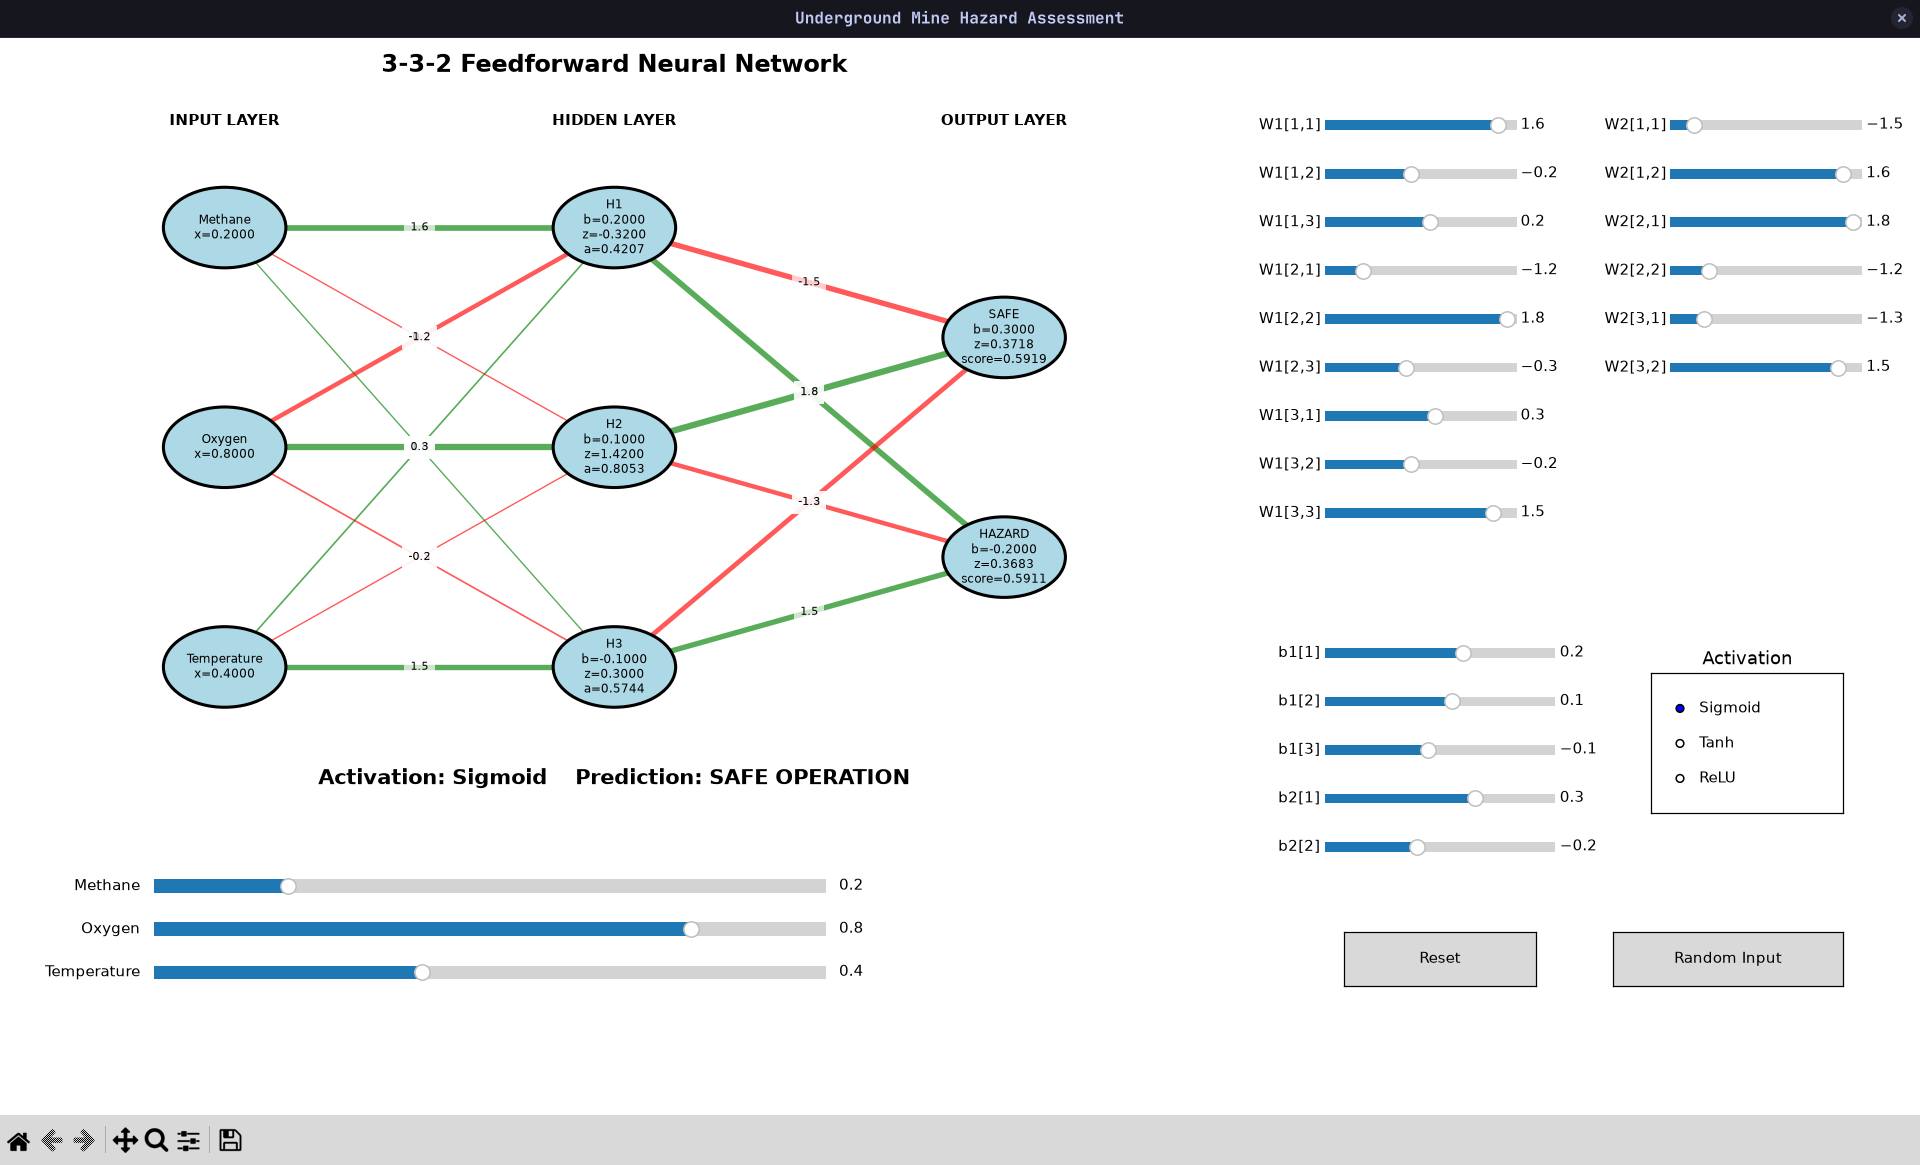
\includegraphics[width=0.95\linewidth]{output.png}
    \caption{Interactive visualization of the underground mine hazard
    assessment neural network.}
    \label{fig:network-output}
\end{figure}

% =================================================
% EXPERIMENTAL ANALYSIS
% =================================================

\section{Experimental Analysis}

\subsection{Effect of Methane Concentration}

To investigate the effect of methane concentration, methane was varied
from $0.00$ to $1.00$, while oxygen availability and ambient
temperature were maintained at

\[
\text{Oxygen}=0.80,
\qquad
\text{Temperature}=0.40.
\]

The default network parameters and Sigmoid activation function were
used.

\begin{table}[H]
\centering
\small
\caption{Effect of methane concentration on network output}
\resizebox{\textwidth}{!}{
\begin{tabular}{ccccccc}
\toprule
Methane & $H_1$ & $H_2$ & $H_3$ &
Safe Score & Hazard Score & Prediction\\
\midrule
0.00 & 0.3452 & 0.8115 & 0.5646 & 0.6245 & 0.5561 & Safe\\
0.10 & 0.3823 & 0.8085 & 0.5695 & 0.6086 & 0.5734 & Safe\\
0.20 & 0.4207 & 0.8053 & 0.5744 & 0.5919 & 0.5911 & Safe\\
0.30 & 0.4601 & 0.8022 & 0.5793 & 0.5746 & 0.6089 & Hazardous\\
0.40 & 0.5000 & 0.7990 & 0.5842 & 0.5569 & 0.6266 & Hazardous\\
0.50 & 0.5399 & 0.7958 & 0.5890 & 0.5391 & 0.6439 & Hazardous\\
0.60 & 0.5793 & 0.7925 & 0.5939 & 0.5214 & 0.6608 & Hazardous\\
0.70 & 0.6177 & 0.7892 & 0.5987 & 0.5039 & 0.6769 & Hazardous\\
0.80 & 0.6548 & 0.7858 & 0.6035 & 0.4870 & 0.6921 & Hazardous\\
0.90 & 0.6900 & 0.7824 & 0.6083 & 0.4707 & 0.7063 & Hazardous\\
1.00 & 0.7231 & 0.7790 & 0.6130 & 0.4553 & 0.7194 & Hazardous\\
\bottomrule
\end{tabular}
}
\end{table}

\subsection{Analysis of Hidden Neurons}

As methane concentration increases, the first hidden neuron's
activation increases significantly from $0.3452$ to $0.7231$.
This occurs because the connection from methane to the first hidden
neuron has a relatively large positive weight of $1.6$.

The second hidden neuron's activation decreases slightly from
$0.8115$ to $0.7790$. This behaviour is caused by the negative
methane-to-hidden connection weight of $-0.2$.

The third hidden neuron's activation increases from $0.5646$ to
$0.6130$ because methane is connected to this neuron using a positive
weight of $0.2$.

Thus, changing a single input can affect different hidden neurons in
different directions depending on the signs and magnitudes of their
connection weights.

\subsection{Analysis of Output Scores}

As methane concentration increases, the Safe Operation score
continuously decreases. It changes from approximately $0.6245$ at
zero methane to $0.4553$ when methane reaches $1.00$.

In contrast, the Hazardous Condition score continuously increases from
approximately $0.5561$ to $0.7194$.

At the default methane concentration of $0.20$, the output scores are

\[
\text{Safe}=0.5919,
\qquad
\text{Hazard}=0.5911.
\]

Therefore, the network predicts Safe Operation, although the two scores
are very close.

At methane concentration $0.30$, the scores become

\[
\text{Safe}=0.5746,
\qquad
\text{Hazard}=0.6089.
\]

The network therefore changes its prediction to Hazardous Condition.
Hence, for the tested values, the change in classification occurs
between methane concentrations $0.20$ and $0.30$.

% =================================================
% OBSERVATIONS
% =================================================

\section{Observations}

The following observations were made during the experiment:

\begin{enumerate}

    \item Changes in environmental sensor inputs propagate through the
    hidden layer before influencing the final output neurons.

    \item The effect of an input on a hidden neuron depends on both the
    sign and magnitude of the corresponding connection weight.

    \item Increasing methane concentration causes the Safe Operation
    score to decrease and the Hazardous Condition score to increase
    for the given network parameters.

    \item The network predicts Safe Operation at the default methane
    concentration of $0.20$, but the two output scores are almost
    equal.

    \item For the methane values tested in increments of $0.10$, the
    prediction changes from Safe Operation to Hazardous Condition
    between methane concentrations $0.20$ and $0.30$.

    \item Changing the activation function modifies the hidden
    activations and output scores because Sigmoid, Tanh, and ReLU
    transform the weighted sums differently.

    \item Positive and negative weights can be visually distinguished
    in the network, while connection thickness provides an indication
    of weight magnitude.

    \item The interactive controls make it possible to directly
    observe the relationship between network parameters and forward
    propagation without performing any training or backpropagation.

\end{enumerate}

% =================================================
% CONCLUSION
% =================================================

\section{Conclusion}

In this experiment, an interactive 3--3--2 feedforward neural network
was implemented to simulate an underground mine hazard assessment
system. Methane concentration, oxygen availability, and ambient
temperature were used as environmental inputs, while the two output
neurons represented Safe Operation and Hazardous Condition.

Forward propagation was implemented using NumPy, while Sigmoid, Tanh,
and ReLU activation functions were provided for interactive selection.
Matplotlib widgets were used to modify the environmental inputs,
connection weights, neuron biases, and activation function during
execution. The resulting weighted sums, activations, output scores,
and final prediction were visualized in real time.

The methane experiment demonstrated how changing a single input
propagates through the hidden layer and subsequently affects the
output scores. With the default parameters and Sigmoid activation,
increasing methane caused the Safe Operation score to decrease,
while the Hazardous Condition score increased.

For the methane concentrations tested, the network predicted Safe
Operation at $0.20$ and Hazardous Condition at $0.30$. Therefore,
the transition in the predicted condition occurs between methane
concentrations $0.20$ and $0.30$.

The experiment therefore provides a clear visualization of the forward
propagation process and demonstrates how neural-network predictions
are determined by the combined effects of inputs, weights, biases, and
activation functions.

\end{document}
